\documentclass[conference]{IEEEtran}
\usepackage{amsmath,amsfonts,amssymb}
\usepackage{graphicx}
\usepackage{color}
%\usepackage{url}

\begin{document}
\title{CS8803-O03 Reinforcement learning\\Project 1 report}

\author{\IEEEauthorblockN{Rohan D. Kekatpure}
\IEEEauthorblockA{Email: rdk@gatech.edu}}
% make the title area
\maketitle

% As a general rule, do not put math, special symbols or citations
% in the abstract
%\begin{abstract}
%\end{abstract}

\IEEEpeerreviewmaketitle
\section{Introduction}
Per our best understanding, Sutton's paper \cite{sutton88} has two main purposes. The first is to advance the TD($\lambda$) family of algorithms as more efficient and more accurate methods for learning in multi-step prediction settings (i.e. where the training data comes in as an ordered sequence of inputs rather than just input-output pairs) and the second is to prove some theorems related to convergence properties of the TD methods. The theorems proved in the latter part of the paper mostly apply to the extreme values $\lambda=0$ or $\lambda=1$. The paper conjectures (without proof) that similar convergence properties may hold for intermediate values $0<\lambda<1$. The veracity of this conjecture is motivated by a computational example of a 5-state random walk. The computational experiments demonstrate that for the right value of the parameters $\alpha$ (the learning rate) and $\lambda$ (the trace decay parameter), the TD($\lambda$) algorithm converges to the value function faster and more accurately. The aim of this report is to outline the implementation of $\text{TD}(\lambda)$ learning algorithm using the random walk experiment as described in sections 2 and 3 of the paper. 
\section{Definitions}
To keep the following presentation clear, we first begin with definitions of various terms.
\begin{enumerate}
\item{\bf Random  walk problem:} The random walk problem is the 5-state problem that appears in Figure 2 in the paper. Specifically the terminal states $A$ and $G$ are absorbing states with rewards $z = 0$ and $z = 1$ respectively. The intervening states $B$, $C$, $D$, $E$, and $F$ each have equal probability (i.e. $\frac{1}{2}$) of transitioning to their left or right neighbor.
%%
\item{\bf Sample:} Sample is an instance of a state. In the random walk problem, a sample is one state chosen from $\{B, C, D, E, F\}$.
%%
\item{\bf Sequence:} A sequence is a series of states, always beginning with the state $D$ and ending in $A$ (with reward 0) or $G$ (with reward 1). Because of the probabilistic transitions, a sequence may have any number of steps (possibly infinite) and the steps may repeat. A sequence can be represented in two ways. First is just as a series of labels and a reward. For example ${DEFEF, z=1}$ is a sequence beginning in $D$ and ending in $G$ with a reward 1. For computations the states can also be mapped to unit column vectors. For example $B = [1, 0, 0, 0, 0]^\intercal$, $C = [0, 1, 0, 0, 0]^\intercal$ and so on. In this representation, the previous sequence can be represented as horizontally-stacked column vector:
\begin{equation*}
\{DEFEF, 1\} =
    \left\{ 
        \begin{bmatrix}
        0 & 0 & 0 & 0 & 0 \\
        0 & 0 & 0 & 0 & 0 \\
        1 & 0 & 0 & 0 & 0 \\
        0 & 1 & 0 & 1 & 0 \\
        0 & 0 & 1 & 0 & 1 
        \end{bmatrix},1
    \right\}
\end{equation*}
The term ``sequence'' is also used interchangeably with the term {\bf walk}, both of which capture a single random walk instance beginning in $D$ and ending in an absorbing state. 
%%
\item{\bf Training set:} A training set is a set of 10 sequences. For example $T = [\{DEFEF, 1\},\{DCB, 0\}, \ldots]$, and $\#\{T\}=10$.
\item{\bf Iteration:} An iteration is one pass of the algorithm through the training set where the training set contains 10 sequences and each sequence has a variable number of steps (transitions). 
\end{enumerate}
%%%%
%%%%
\section{Implementation}
Our implementation is based on Equations (1) and (4) of the paper supplemented by the equation for evolution of the eligibility trace. We reproduce them for completeness below taking account of the fact that we're using a linear model for predictors. This is also how we have translated them into code.
\begin{align}
P_t &= w^\intercal x_t \label{eq:linmod}\\
\Delta w_t &= \alpha(P_{t+1} - P_t)e_t \\
e_{t+1} &= x_{t+1} +\lambda e_t\\
w &\leftarrow w + \sum_{i=1}^n\Delta w_t\\
\text{RMSE} &= \sqrt{\frac{\sum_{i=1}^5(w_i - W_i)^2}{n}},
\end{align}
where $W = [0.167, 0.334, 0.500, 0.667, 0.834]$ are the theoretically calculated true weight vectors. In the first experiment, the weights are updated after learning on the full training set (containing 10 sequences). In the second experiment, the updates are performed after learning on each sequence. Note that a linear model, Eq.~\eqref{eq:linmod}, readily provides the gradient $\nabla_wP_t = x_t$. One has to be careful to deal properly with the {\bf edge cases}. Assuming, $t$ for the given sequence runs from 1 to $m$, we define $P_{m+1} = z$ and only calculate the quantities $\Delta w_t$ and $e_t$ from 1 through $m$. The weight vector is initialized to $w=[0.5, 0.5, 0.5, 0.5, 0.5]^\intercal$ and $x_1 = e_1 = [0,0,1,0,0]^\intercal$ is defined before the run. We took no special measures to deal with {\bf repeated states}. We found that for $\alpha<0.025$ (on a 0.05 search grid), repeated states don't cause any divergence even for sequences with several dozen steps.
%%%%
%%%%
\section{Results and discussion}
\subsection{Experiment 1: Batch update}
In the first experiment, the weights are updated only after encountering the entire 10-sequence training set. The procedure is repeated with the same training set until the weights converge. Weights are said to have {\bf converged} when the RMS difference between the old weight vector and the new weight vector is less than 0.01. Figure~\ref{fig:expt1} shows the results of our experiment in the batch mode. The parameters used for this experiment are listed in the caption. Particularly, the learning rate $\alpha = 0.025$ was kept constant. This is the largest learning rate which led to a stable convergence. The weights for $\lambda = 1$ diverged for $\alpha = 0.03$. The numbers on the $y$-axis of Figure~\ref{fig:expt1} don't match with those in Figure~3 in the paper. Whereas in the corrected version of Figure~3 in the paper, the error varies between 0.19 and 0.25 as $\lambda$ varies between 0 to 1, the corresponding range of error in our experiments is from 0.09 to 0.17. 

The numeric difference in Figure~\ref{fig:expt1} and Figure~3 in the paper is caused by the sensitivity of the error figures to the the parameters of the simulation, particularly the learning rate $\alpha$. Sutton's paper unfortunately doesn't mention the exact value learning rate used to generate Figure~3 nor the sensitivity of his results to the parameter. 

The main objective of the study, however, is to demonstrate that TD($\lambda<1$) and TD(1) (Widrow-Hoff) procedures converge to a different set of weights since they minimize different objective functions. The Widrow-Hoff procedure minimizes the error on the training set and the TD(0) converges to the expected state rewards. This trend is identical to the paper; the RMS difference drops down drastically as $\lambda$ is decreased from 1 toward 0. The {\bf error bars} on the plots denote the standard error (SE) for each $\lambda$ calculated from the list of RMS errors (obtained from running the training procedure on 100 training sets): $\text{SE} = \sigma/\sqrt{n}$ where $n = 100$. As confirmed by Sutton, $\text{SE}<0.01$; the differences in the converged value functions are indeed {\bf statistically significant}.
%%
\begin{figure}[!bt]
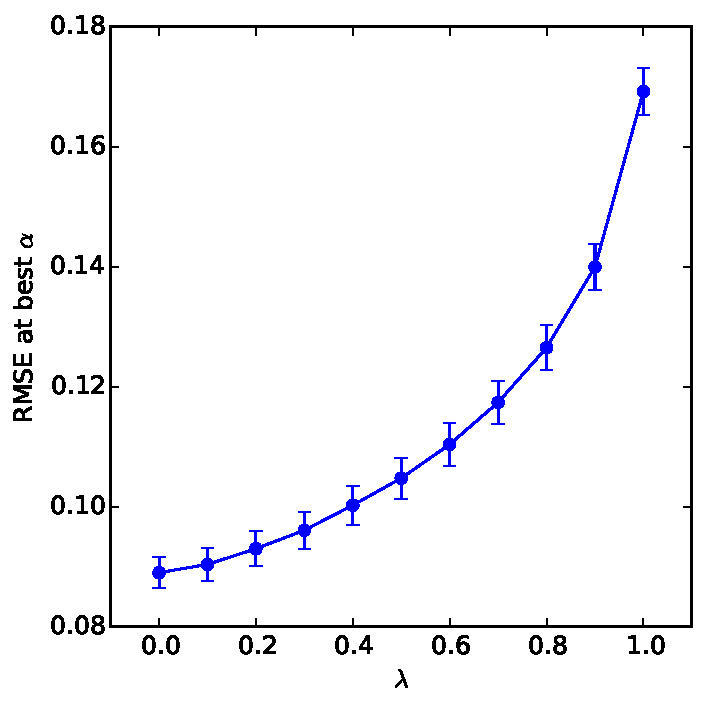
\includegraphics[width=0.5\textwidth]{./figures/fig3.pdf}
\caption{Comparison of TD($\lambda$) algorithms for batch learning (Figure 3 in Sutton88 paper). The error bars denote the standard error and are calculated as $\text{SE} = \sigma/\sqrt{n}$. The parameters for this simulation are: $\alpha = 0.025$, number of training sets $n = 100$.\label{fig:expt1}}
\end{figure}
%%
\subsection{Experiment 2: Online update}
Experiment 1 demonstrated that TD($\lambda$) algorithms converge to the value functions when trained in batch mode. However often the entire dataset isn't available {\em apriori}. The algorithms are forced to learn from data stream. This is the realm of {\bf online} learning. The second experiment in Sutton's papers concerns the comparison of convergence behavior of TD($\lambda$) family of algorithms in an online setting. We use the same training sets as before, but now update the weights after training on every sequence in the training set. Since the training set here consists of 10 sequences, there will be 10 weight updates while training on a single training set. 
%%
\begin{figure}[!bt]
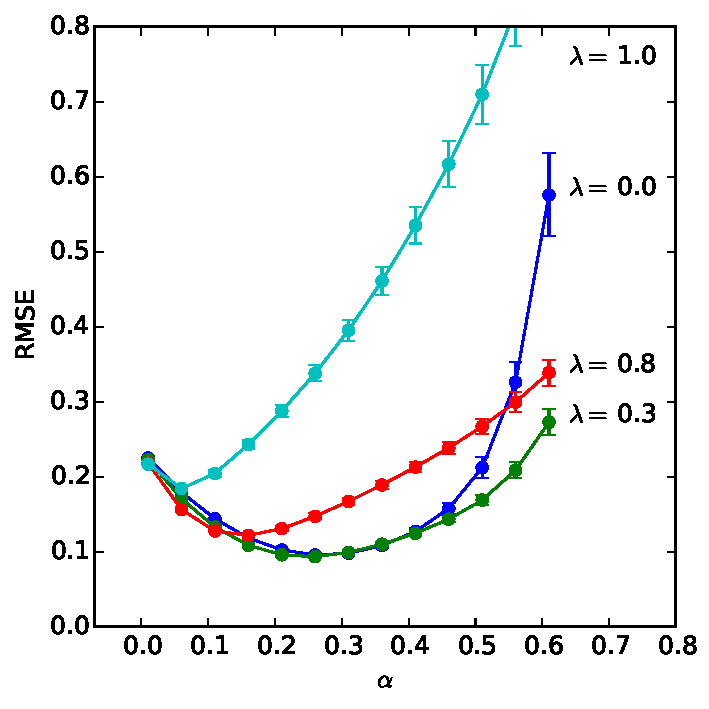
\includegraphics[width=0.5\textwidth]{./figures/fig4.pdf}
\caption{Comparison of TD($\lambda$) algorithms for online learning (Figure 4 in Sutton88 paper). Each point represents an average over 100 training set. The standard error $\text{SE} = \sigma/\sqrt{n}$ where $n=100$ and $\sigma$ is the standard deviation of the 100 RMSE values.\label{fig:expt2a}}
\end{figure}
%%

The results depicted in Figure~\ref{fig:expt2a} are very similar to Figure~4 in Sutton's paper. The results are very sensitive to the learning rate $\alpha$ and the best estimates (i.e. closest to theoretical values) are obtained for $0.1 \leqslant \alpha \leqslant 0.4$. The Widrow-Hoff or the TD(1) procedure diverges with increasing $\alpha$  and produces the worst estimates. TD($\lambda$) for $\lambda = 0$ and $0.3$ produce best estimates and are stable around a broad range of $\alpha$ values. 

To find the $\lambda$ value that produces the best estimates, we plot the minimum error for each $\lambda$ value. This is plotted in Figure~\ref{fig:expt2b}. From the figure we can conclude that the best RMS error is obtained for $\lambda=0.2$. More importantly, the algorithm is stable around that value. That is, small variations of the $\lambda$ values around the best value won't cause wild changes parameter estimates. 
%%
\begin{figure}[!bt]
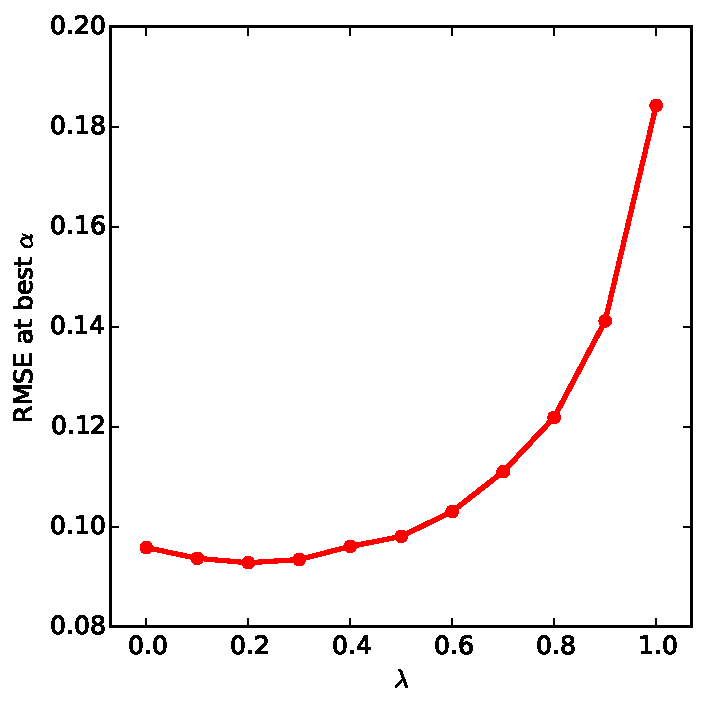
\includegraphics[width=0.5\textwidth]{./figures/fig5.pdf}
\caption{Comparison of TD($\lambda$) algorithms for online learning (Figure 5 in Sutton88 paper). For each given $\lambda$ we select the minimum RMS error of the corresponding curve on Figure~\ref{fig:expt2a}. Error bars are too small to be visible, so the results are statistically significant.\label{fig:expt2b}}
\end{figure}
%%
\section{Comparison to similar calculations}
The 5-state, single-reward problem is presented in detail in Chapter 6 of the Sutton/Barto book \cite{suttonbarto}. Although not presented in the main body of this report, we observed several of the artifacts of the TD calculations presented in Figure~6.7 of the book. Particularly, with smaller values of the learning rate ($\alpha \leq0.025$) lead to more stable and accurate convergence, but it is slow. Larger values ($\alpha\geq0.1$) lead to faster convergence, but they're less accurate and prone to divergence as the number of walks/episodes increases. Larger $\alpha$ values also make walks with {\bf repeated states} more unstable for higher $\lambda$ values. This happens because of a repeated encounter of a state whose eligibility hasn't yet decayed enough. 
%%
\section{Theoretical calculation of value function}
Equation~(5) in Sutton's paper provides an explicit formula for calculating expected returns from every state (i.e. the value function). However, we found that the theoretical weights can also be calculated by simple logical reasoning as presented below. 

First, recognize that the transition probabilities are symmetric about state $D$. That is, the transition probability from $B$ to $A$ is same as that from $F$ to $G$ and so on. Therefore we're working with only three probabilities $p_1$, $p_2$, and $p_3$ as shown in Figure~\ref{fig:markov}. Further, since $D$ has an equal probability of landing in $G$ or $A$ and since it eventually must end in one, $2p_3 = 1\Rightarrow p_3=\frac{1}{2}$.

With reference to the bottom left transition diagram in Fig.~\ref{fig:markov}, there are two ways from $F$ to $G$: direct, with a probability $\frac{1}{2}$ and through $E$ with probability $\frac{1}{2}p_2$. The total probability of landing in $G$ from $F$ is the sum of these two: $p_1 = \frac{1}{2} + \frac{1}{2}p_2$. Similarly, with reference to the transition diagram in the bottom-right, we can write for $E$: $p_2 = \frac{1}{2}p_1 + \frac{1}{2}p_3$. Substituting $p_3=\frac{1}{2}$ and solving for $p_1$ and $p_2$ yields $p_1=\frac{5}{6}$ and $p_2=\frac{2}{3}$. Transition probabilities from $B$ and $C$ to $G$ are $1-p_1 = \frac{1}{6}$ and $1-p_2 = \frac{1}{3}$ respectively. This completes the calculation.
%%
\begin{figure}[!bt]
\centering
\includegraphics[width=3in]{./figures/markov.png}
\caption{Computation of theoretical weights. The top part of the figure defines the various transition probabilities. The bottom left and right figures are the transition diagrams for state $F$ and $E$ respectively.\label{fig:markov}}
\end{figure}
%%
\section*{Conclusion}
To summarize, we successfully reproduced computer experiments in Sutton's 1988 paper. Since the results of experiment 1 are highly sensitive to the value of the learning rate $\alpha$, there is a slight numerical difference between our results and Sutton's. However, the trends and conclusions are identical. Results of experiment 2 are more close visual and numerical match to the paper. 
\begin{thebibliography}{1}
\bibitem{sutton88}
Richard~S.~Sutton, {\em Machine Learning}, {\bf 8} p. 9--44, 1988.
\bibitem{suttonbarto}
Richard~S.~Sutton and Andrew~G.~Barto, ``Reinforcement Learning,'' {\em MIT Press}, 1998.
\end{thebibliography}

\end{document}


